\documentclass{article}
\usepackage[T1]{fontenc}
\usepackage[latin1]{inputenc}
\usepackage[margin=2.25cm,headheight=26pt,includeheadfoot]{geometry}
\usepackage[english]{babel}
\usepackage{listings}
\usepackage{color}
\usepackage{titlesec}
\usepackage{titling}
\usepackage[framed, numbered]{matlab-prettifier}
\usepackage{changepage}
\usepackage{amsmath}
\usepackage{hyperref}
\usepackage{enumitem}
\usepackage{graphicx}
\usepackage{fancyhdr}
\usepackage{lastpage}
\usepackage{caption}
\usepackage{tocloft}
\usepackage{setspace}
\usepackage{multirow}
\usepackage{titling}
\usepackage{float}
\usepackage{comment}
\usepackage{booktabs}
\usepackage{indentfirst}
\usepackage{lscape}
\usepackage{booktabs,caption}
\usepackage[flushleft]{threeparttable}
\usepackage[english]{nomencl}
\usepackage{xcolor}
\usepackage{lipsum}


% --- set footer and header ---
\pagestyle{fancy}
\fancyhf{}

\setlength{\parindent}{2em}
\title{Stock Performance of LQ45 Index} % to reference as \title, dont use \maketitle
\makeatletter\let\Title\@title\makeatother



\lstset{language=Matlab,
style=Matlab-editor,
basicstyle=\normalsize\mlttfamily,
numbers=left,
numberstyle={\scriptsize\color{black}},			% size of the numbers
numbersep=0.5cm											
}
}

\newlist{steps}{enumerate}{1}
\setlist[steps, 1]{leftmargin=1.5cm,label = Step \arabic*:}
\renewcommand{\headrulewidth}{1pt}
\renewcommand{\footrulewidth}{1pt}
\renewcommand{\rmdefault}{ptm}

%\lhead{\Title}
\rhead{\nouppercase{\rightmark}}
\lhead{\Title}
\rfoot{
\includegraphics[height=1.5cm]{root/IITMD.png}} % right header logo
\setlength\headheight{16pt}
\setlength{\footskip}{50pt}
\lhead{\Title} %rightH title
\cfoot{\thepage}

% --- End of page settings ---



\begin{document}
\pagenumbering{Roman} 
\begin{titlepage}
\begin{center}
\vspace{2cm}
%\textsc{ Oregon State University}\\[1.5cm]

\includegraphics[width=0.4\textwidth]{root/IITMD.png}~\\[1cm]
\vspace{1cm}

% Title
\hrule
\vspace{.5cm}
{ \huge \bfseries Report on\\ STOCK PERFORMANCE OF LQ45 INDEX} % title of the report
\vspace{.5cm}

\hrule
\vspace{1.5cm}

\textsc{\textbf{Authors}}\\
\vspace{.5cm}
\centering

% add your name here
Bhavik Ostwal - B23395\\
Yadnyit Panchbhai - B23477\\
Gaurav Yadav - B23398\\
Dheeraj Jha - B23369\\
Hardeep Gupta - B23015\\
Lalit Kishore - B23352\\

\vspace{4cm}

\centering \today % Dags dato
\end{center}
\end{titlepage}

\newpage
\doublespacing
\addcontentsline{toc}{section}{Table of Contents}
\renewcommand{\baselinestretch}{1}\normalsize
\tableofcontents

\renewcommand{\baselinestretch}{1}\normalsize
%\singlespacing
\thispagestyle{fancy} % force page style


\newpage
\pagenumbering{Roman}
\fancyfoot[C]{Page \thepage\ of \pageref{endOfDoc}}

\section{Introduction} \label{ch1}

\par

In the wake of the COVID-19 pandemic, Indonesia is witnessing a compelling economic resurgence marked by a resurgence in foreign investment inflows into its capital market.

Intrigued by the shifting tides of economic fortune, our analysis delves into the comparative landscape of stock returns before and during the pandemic era. Focusing on the esteemed LQ45 index, a curated selection of blue-chip stocks reflective of Indonesia's market pulse, we traverse the years 2017 to 2021 to uncover nuanced insights.

In this journey, we zoom in on the financial sector, a cornerstone of market capitalization, chosen for its inherent dynamism and resilience. By juxtaposing pre-pandemic performance with the pandemic era, we aim to unveil the intricate dance of risk and reward that shapes investor sentiment and market trajectories.

Stock investing is a popular method for building wealth over the long term. One of the primary reasons investors choose to invest in stocks is the potential for attractive returns. In this report, we will explore the concept of stock investing returns, including what they are, how they are calculated, factors influencing returns, and strategies for maximizing returns while managing risks.

\subsection{Objectives}
\begin{enumerate}
    \item To analyze the difference in stock investing returns in the pre-pandemic (2017-
2019) and during the pandemic (2020-2021) on LQ45 stocks.
    \item To analyze the difference in stock investing risks in the pre-pandemic (2017-
2019) and during the pandemic (2020-2021) on LQ45 stocks.
\end{enumerate}

% \begin{figure}[H]
    % \centering
    % \includegraphics[width = 0.2\textwidth ]{figures/tex.png}
    % \caption{Increase of battery capacity. \cite{china_too_many}}
    % \label{fig:batteryIncreas}
% \end{figure}

% \subsection{Questions}
% \begin{enumerate}
%     \item Is there any difference in stock investing returns between the pre-pandemic
% (2017-2019) and during the pandemic (2020-2021) on LQ45 stocks?
%     \item Is there any difference in stock investing risks between the pre-pandemic
% (2017-2019) and during the pandemic (2020-2021) on LQ45 stocks?
% \end{enumerate}


% \begin{table}[H]
%     \centering
%     \caption{That is a table.}
%     \begin{tabular}{|c|c|c|}
%     \centering

%     \end{tabular}
%     \label{tab:table1}
% \end{table}

 

\label{EndOfText}


\newpage
\fancyfoot[C]{Page \thepage\ of \pageref{endOfDoc}}
\section{Mechanics} \label{ch2}


\subsection{Qualitative Data}
\par
In the dynamic landscape of stock markets, fundamental analysis plays a pivotal role in understanding the nuances of stock performance. This report delves into the qualitative aspects of the LQ45 index companies, focusing on the categorization of these entities into state-owned and private-owned enterprises from 2017 to 2021.

\begin{table}[H]
    \centering
    
    \caption{Type of the company listed in LQ45 2017 - 2021}
    
    \centering
    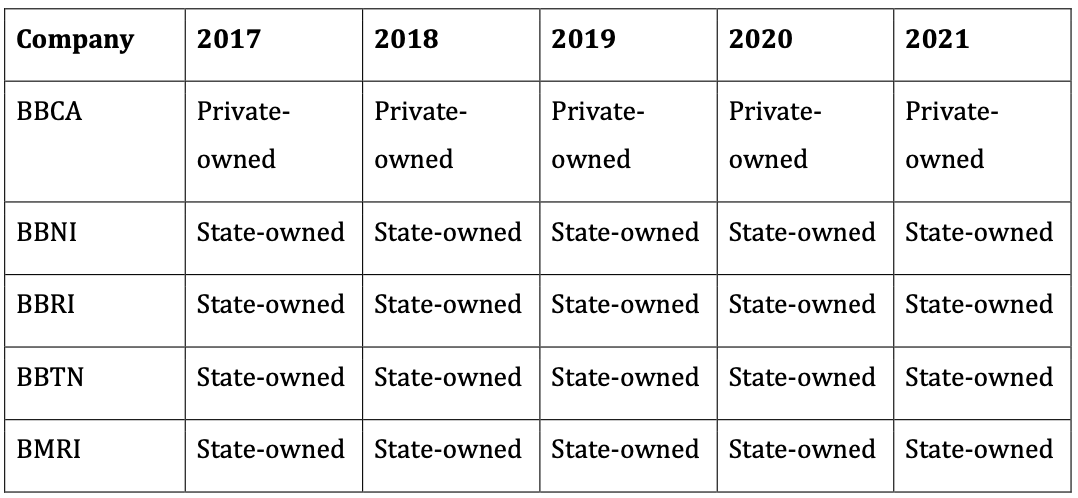
\includegraphics[width = 0.8\textwidth]{figures/table_1.png}
    \label{tab:}
\end{table}

\paragraph{Conclusion:}
\par The qualitative analysis of the LQ45 index companies underscores the enduring dominance of state-owned enterprises and the consequential implications for stock performance. By delving into ownership structures and profitability dynamics, this report provides valuable insights for investors, policymakers, and stakeholders navigating the complexities of the stock market.

\subsection{Quantitative Data}

This section delves into the quantitative data derived from monthly closing stock prices of prominent companies within the LQ45 index, namely BBCA, BBNI, BBRI, BBTN, and BMRI. Through the calculation of monthly stock returns, we unravel the patterns and trends shaping the investment landscape.

Data used in this report is in the form of monthly closing stock prices which are then processed to obtain the monthly stock returns of BBCA, BBNI, BBRI, BBTN, and BMRI using the formula:

$$
\text{Return}_{t} = \frac{\text{Closing Price}_{t} - \text{Closing Price}_{t-1}}{\text{Closing Price}_{t-1}}
$$

\begin{figure}[H]
    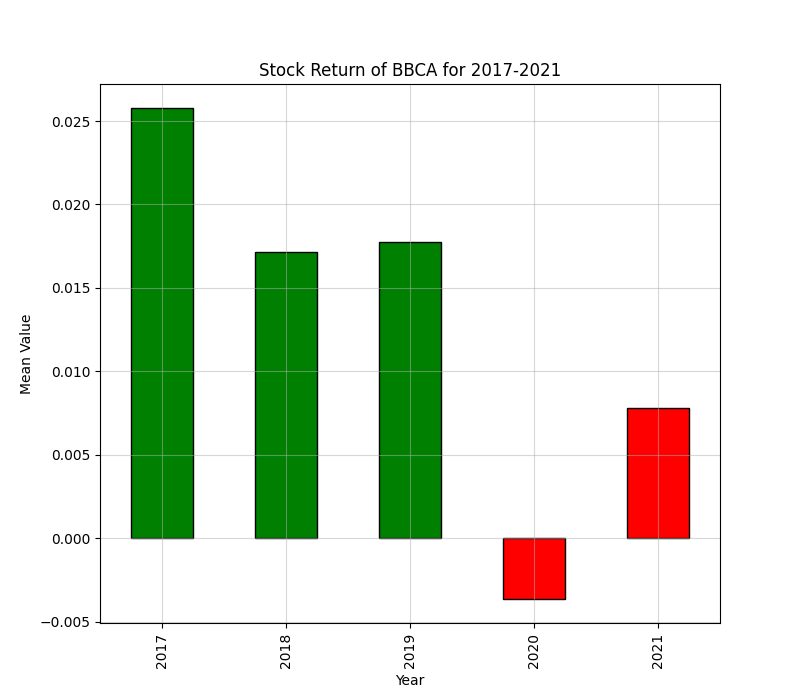
\includegraphics[width = .55\textwidth ]{figures/BBCA.png}
    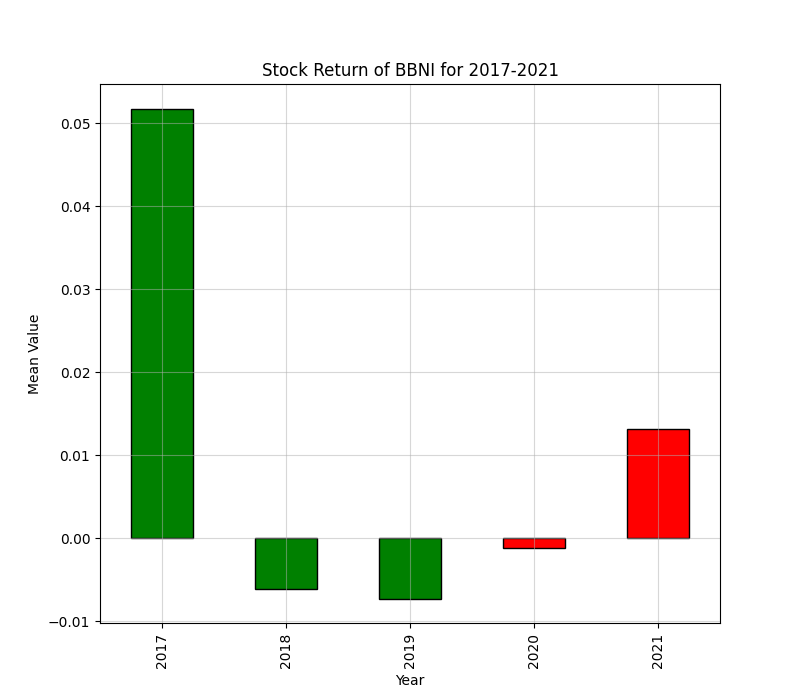
\includegraphics[width = .55\textwidth ]{figures/BBNI.png}
\end{figure}

\begin{figure}[H]
    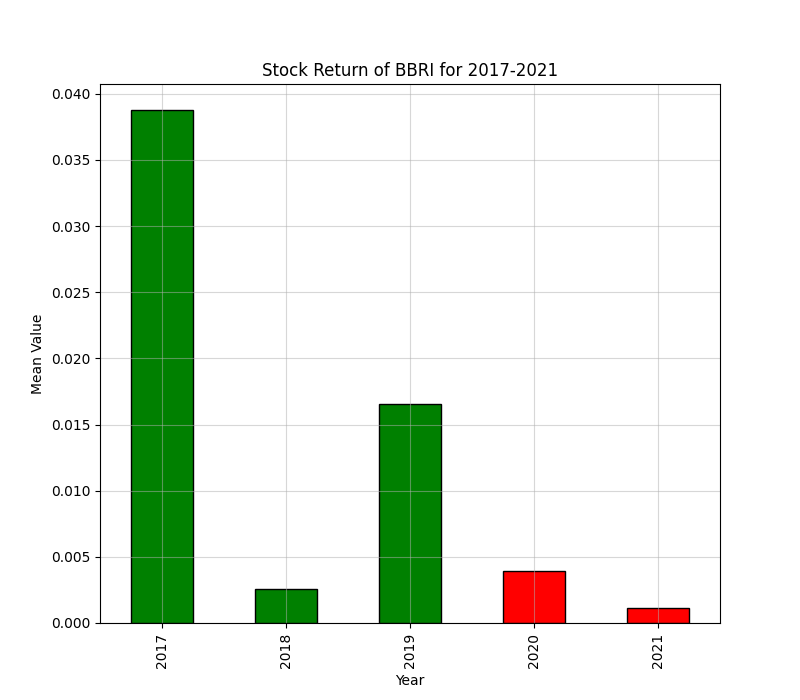
\includegraphics[width = .55\textwidth ]{figures/BBRI.png}
    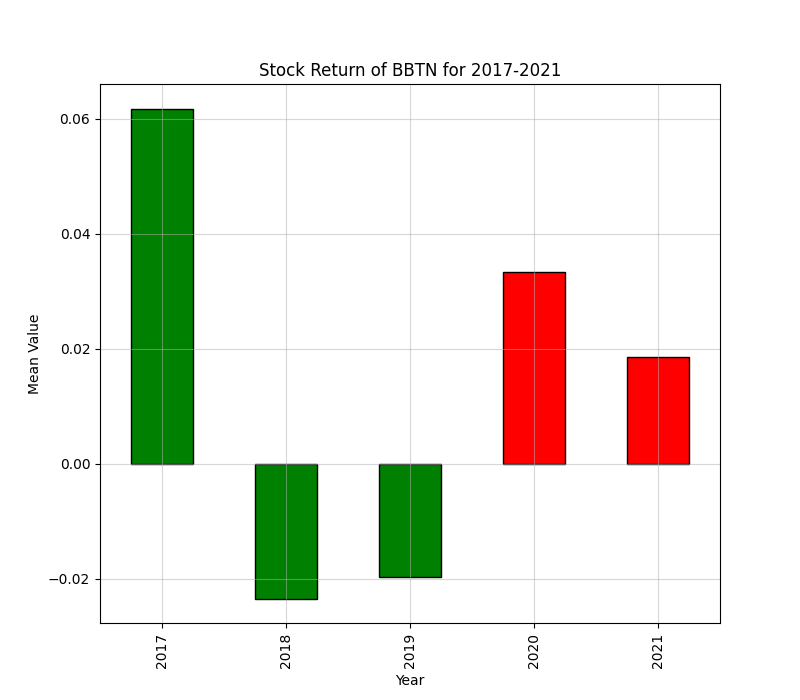
\includegraphics[width = .55\textwidth ]{figures/BBTN.png}
\end{figure}

\begin{figure}[H]
    \centering
    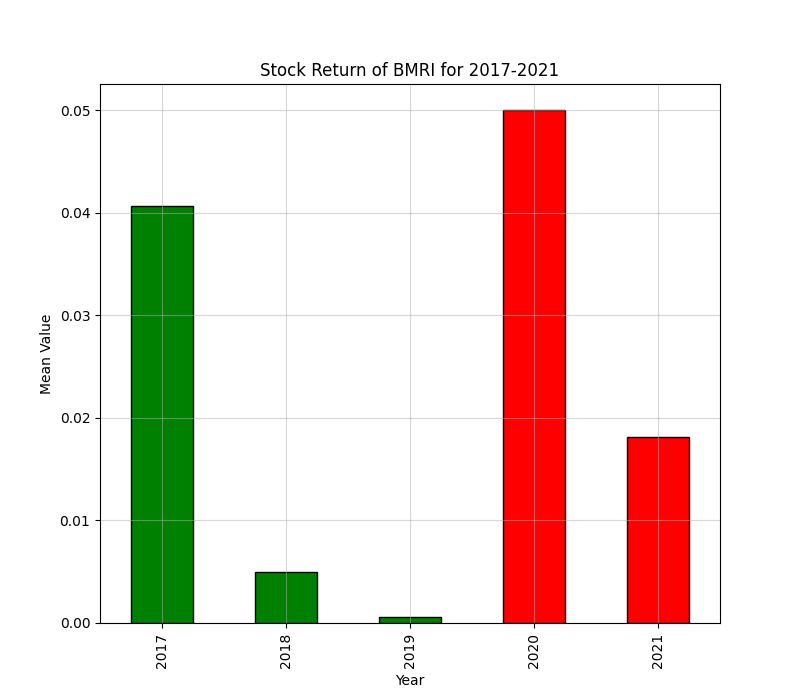
\includegraphics[width = .55\textwidth ]{figures/BMRI.png}
\end{figure}

\paragraph{Conclusion:}
\par The quantitative analysis of monthly stock returns provides valuable insights into the performance dynamics of selected companies within the LQ45 index. By leveraging quantitative data, investors can make informed decisions, optimize investment strategies, and navigate the complexities of the stock market with confidence.







 

\label{EndOfText}


\newpage
\fancyfoot[C]{Page \thepage\ of \pageref{endOfDoc}}
\section{Stock Investing Returns} \label{ch3}
\subsection{What are Stock Investing Returns?}
Stock investing returns refer to the profits or losses generated by investing in stocks over a specific period. These returns are typically expressed as a percentage and reflect the performance of an investment relative to its initial cost.

\subsection{Calculating Stock Returns}
The formula for calculating stock returns is:
\[ \text{Stock Return} = \left( \frac{\text{Current Stock Price} - \text{Initial Stock Price} + \text{Dividends}}{\text{Initial Stock Price}} \right) \times 100\% \]

\subsection{Factors Influencing Stock Returns}
Several factors influence stock returns, including:
\begin{itemize}
    \item Market Conditions
    \item Company Performance
    \item Industry Trends
    \item Dividends
    \item Market Sentiment
\end{itemize}

\subsection{Strategies for Maximizing Returns}
Investors employ various strategies to maximize stock investing returns, including:
\begin{itemize}
    \item Diversification
    \item Long-Term Investing
    \item Research and Analysis
    \item Risk Management
    \item Reinvestment of Dividends
\end{itemize}

\subsection{Conclusion}
Stock investing returns are a key consideration for investors seeking to grow their wealth in the financial markets. By understanding the factors influencing returns and employing effective investment strategies, investors can potentially achieve attractive long-term returns while managing risks effectively.

% \section{References}
% \begin{enumerate}
%     \item Investopedia: \texttt{https://www.investopedia.com/terms/s/stockreturn.asp}
%     \item The Balance: \texttt{https://www.thebalance.com/how-to-calculate-stock-returns-4683693}
%     \item Forbes: \texttt{https://www.forbes.com/sites/forbesfinancecouncil/2020/06/01/5-strategies-to-maximize-your-investment-returns/?sh=5f13704f7fc9}
% \end{enumerate}

 

\label{EndOfText}


\newpage
\fancyfoot[C]{Page \thepage\ of \pageref{endOfDoc}}
\section{Stock Investing Risks} \label{ch4}
\subsection{What are Stock Investing Risks?}
Stock investing risks include market volatility, company-specific risks such as poor management or industry downturns, and economic factors like inflation or interest rate changes.

\subsection{Calculating Stock Risks}
There isn't a single formula for calculating all stock investing risks, but there are various methods and models such as standard deviation for volatility, beta for market risk, and fundamental analysis for company-specific risks.

\subsection{Factors Influencing Stock Risks}
Several factors influence stock risks, including:
\begin{itemize}
    \item Market Volatility
    \item Company-specific management
    \item Economic Conditions
    \item Industry Trends
    \item Global Events
\end{itemize}

\subsection{Strategies for Minimizing Risks}
Strategies for minimizing stock investment risks include diversification by spreading investments across different assets or sectors, conducting thorough research before investing, setting stop-loss orders to limit losses, and employing risk management techniques like dollar-cost averaging or investing in low-cost index funds.

\subsection{Conclusion}
Stock investing returns are a key consideration for investors seeking to grow their wealth in the financial markets. By understanding the factors influencing returns and employing effective investment strategies, investors can potentially achieve attractive long-term returns while managing risks effectively.

% \section{References}
% \begin{enumerate}
%     \item Investopedia: \texttt{https://www.investopedia.com/terms/s/stockreturn.asp}
%     \item The Balance: \texttt{https://www.thebalance.com/how-to-calculate-stock-returns-4683693}
%     \item Forbes: \texttt{https://www.forbes.com/sites/forbesfinancecouncil/2020/06/01/5-strategies-to-maximize-your-investment-returns/?sh=5f13704f7fc9}
% \end{enumerate}

 

\label{EndOfText}


\newpage
\addcontentsline{toc}{section}{List of Tables}
\listoftables
\thispagestyle{fancy}



\newpage
\addcontentsline{toc}{section}{References}
\bibliography{document.bib} 
\bibliographystyle{ieeetr}


\label{endOfDoc}
\end{document}
